\begin{figure*}
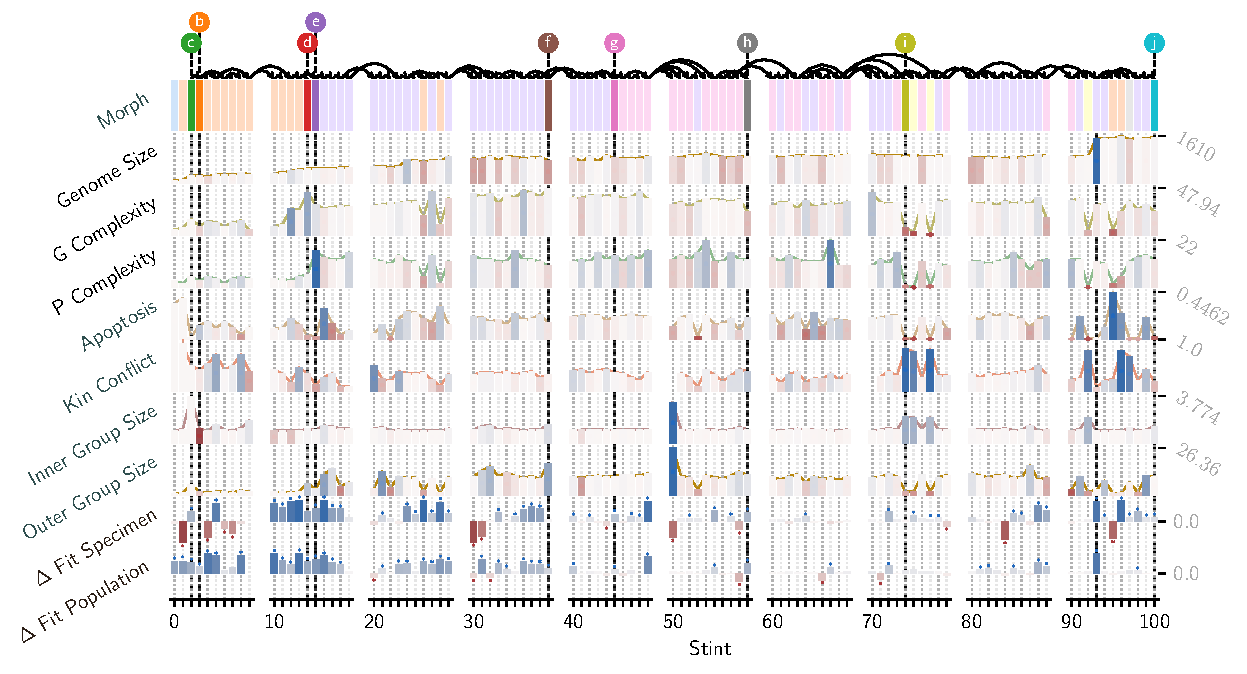
\includegraphics[width=\linewidth]{binder-2025-08-24-keyfig/binder/teeplots/2025-08-24-keyfig/bbg=Contemporary+viz=subplots+ext=.pdf}
\caption{%
\textbf{Overview of complexity, novelty, and adaptation (contemporary biotic background) across evolutionary history.}
\footnotesize
Columns correspond to 100 specimens sampled at sequential checkpoints across evolutionary history (``stints''), arranged left to right.
Top row, ``Morph,'' reports qualitative categorization of multicell structure for sampled specimens.
Arrows indicate estimated ancestry among specimens.
Middle rows trace evolution of individual traits across sampled specimens.
G complexity is genetic complexity --- the number of genome sites with detectable fitness effects in knockout experiments.
P complexity is phenotypic complexity --- the number of distinct cell input/output interfaces that cause fitness loss when disrupted.
Group size, apoptosis, and kin conflict were measured in a monoculture trial.
Bar color-coding indicates magnitude of change relative to ancestor (dark blue as strong positive; dark red as strong negative).
Bottom two rows, ``$\Delta$ Fit Specimen'' and ``$\Delta$ Fit Population'' report fitness competitions between current checkpoint and preceding checkpoint.
In specimen assays, sampled specimen from current checkpoint was competed against a whole-population sample from the preceding checkpoint.
In population assays, whole-population sample from current checkpoint was competed against whole-population sample from the preceding checkpoint.
Positive results indicate fitness gain; negative results indicate fitness loss; asterisks indicate significance ($p < 0.005$).
Fitness assays with contemporary biotic background shown; Figure \ref{fig:keyfig} shows corresponding fitness results without biotic background.
}
\label{fig:keyfig-Contemporary}
\end{figure*}
